\documentclass[11pt,a4paper]{article}

\usepackage[T1]{fontenc}
\usepackage[utf8]{inputenc}
\usepackage{lmodern}
\usepackage{microtype}
\usepackage[margin=2.4cm]{geometry}
\usepackage{amsmath,amssymb}
\usepackage{booktabs}
\usepackage{xcolor}
\usepackage{tikz}
\usetikzlibrary{arrows.meta,positioning,fit,calc,shapes.misc}
\usepackage{pgfplots}
\pgfplotsset{compat=1.18}
\usepackage[numbers,sort&compress]{natbib}
\usepackage{hyperref}
\hypersetup{colorlinks=true,linkcolor=teal!60!black,citecolor=teal!60!black,urlcolor=teal!60!black}
\usepackage{caption}
\captionsetup{font=small,labelfont=bf}
\usepackage{enumitem}
\setlist{itemsep=2pt,topsep=4pt}

\definecolor{qkteal}{HTML}{1F6F78}
\definecolor{qklight}{HTML}{8CC5CB}
\definecolor{qkgrey}{HTML}{9AA3AB}
\definecolor{qkred}{HTML}{B4432F}
\definecolor{qkamber}{HTML}{C98A1B}

\newcommand{\qk}{QuipKeys}
\newcommand{\ttw}[1]{\texttt{#1}}

\newcommand{\ModFix}{77.3}
\newcommand{\ModFixPlain}{53.5}
\newcommand{\BlindNone}{61.7}
\newcommand{\BlindAcc}{89.0}


\title{\qk: Decoding Imprecise Physical-Keyboard Typing\\[4pt]\large Extended report: system, simulated and real-typing evaluation,\\and what a neural language model does and does not add}
\author{Hasnat\\[2pt]\small\url{https://github.com/codinghasnat/quipkeys}}
\date{November 2026}

\begin{document}
\maketitle

\begin{abstract}
Phone keyboards decode where a finger probably meant to land; physical keyboards still rely on conservative dictionary autocorrect. \qk{} is an offline decoder for physical-keyboard typing whose goal is that a person can type fast and imprecisely, without looking at the keys and without backspace, and still get the words they meant.

It combines four parts:
\begin{itemize}[leftmargin=1.2em]
\item an error model of keyboard slips;
\item a weighted edit-distance search over a dictionary trie;
\item an interpolated trigram language model built from 1.4 billion words;
\item a sliding-window lattice decoder, whose confidence in a correction is that correction's posterior probability summed over all decoding paths.
\end{itemize}
Safety mechanisms hold false corrections to about one in 750 correctly typed words. It also repairs misplaced spaces, whole-hand shifts, Shift-key slips and accidental Caps Lock, and switches automatically to a rough-aim error model when the typist is sloppy.

On held-out simulated typing it fixes \ModFix\% of mistyped words at moderate error rates (a frequency-only spellchecker: \ModFixPlain\%), and lifts word accuracy for blind typing (10\% of letters wrong) from \BlindNone\% to \BlindAcc\%. On 33 passages of real, blind, no-backspace typing by one participant at a median of 85~WPM, words typed exactly right rose from 75.4\% to 91.5\%, and 92.5\% with a fitted personal error model. The real data overturned two simulator assumptions, and made keyboard geometry irrelevant for this typist.

Finally, a 23M-parameter neural language model, trained in three hours on a consumer GPU to a perplexity of 59, gave at most +0.3 points. The errors that remain lack \emph{information}, not model capacity, and we discuss what could supply it.
\end{abstract}

\tableofcontents
\bigskip

%=====================================================================
\section{Introduction}

Typing accurately is slow. A large share of everyday keystrokes are spent on correction, even for fast typists~\citep{dhakal2018}: noticing an error, backspacing over it, retyping. Watching for errors also pulls attention from what one is writing.

Touchscreens solved a harder version of the problem. A finger on glass has no key boundaries, so phone keyboards treat each tap as noisy evidence and decode the intended words with a language model~\citep{goodman2002,kristensson2004,vertanen2015}. Physical keyboards never made that transition. Desktop autocorrect, in the operating system or the word processor, is still a cautious dictionary spellchecker: it fixes \ttw{teh}, but it does not reason about which key a finger meant, rarely uses context, and does not repair spacing.

\paragraph{The north star.} The target user does not care where their fingers land. There is intent, but each press lands only roughly near the intended key, and they never look down or backspace. The metric that matters is \emph{effective words per minute}: correct words per minute after all corrections. Figure~\ref{fig:example} shows the kind of input the system must handle.

\begin{figure}[h]
\centering
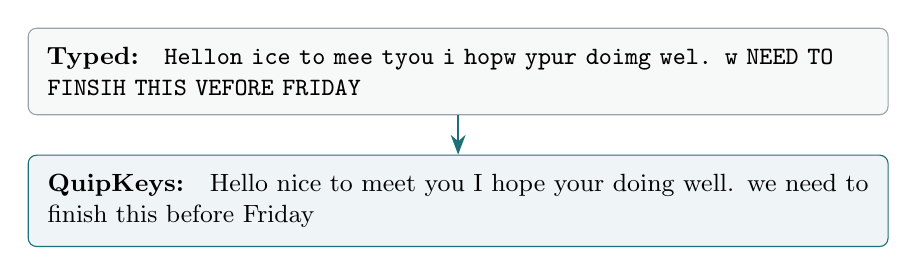
\begin{tikzpicture}[font=\small]
\node[draw=qkgrey,rounded corners=3pt,inner sep=7pt,fill=qkgrey!8,text width=0.86\linewidth] (a) {\textbf{Typed:}\quad \ttw{Hellon ice to mee tyou i hopw ypur doimg wel. w NEED TO FINSIH THIS VEFORE FRIDAY}};
\node[draw=qkteal,rounded corners=3pt,inner sep=7pt,fill=qkteal!7,text width=0.86\linewidth,below=0.5cm of a] (b) {\textbf{\qk:}\quad Hello nice to meet you I hope your doing well. we need to finish this before Friday};
\draw[-{Stealth[length=2.5mm]},thick,qkteal] (a) -- (b);
\end{tikzpicture}
\caption{Spacing slips (\ttw{Hellon ice}, \ttw{mee tyou}), adjacent-key slips (\ttw{hopw}, \ttw{ypur}), a missing letter (\ttw{wel}) and accidental Caps Lock are all repaired. \ttw{your} stays: it is a real word, and the grammar fix (\emph{you're}) is out of scope.}
\label{fig:example}
\end{figure}

\paragraph{Contributions.}
\begin{enumerate}[leftmargin=1.5em]
\item A complete offline decoder for physical keyboards, in Rust, at about 1~ms per word (\S\ref{sec:system}).
\item Safety mechanisms against the failure that makes people turn correction off: changing what they meant (\S\ref{sec:safety}).
\item Repairs that word-level spellcheckers cannot make: spaces, hand shifts, Shift slips, Caps Lock (\S\ref{sec:special}).
\item A five-level benchmark with a simulated typist, including Gaussian ``rough aim'' (\S\ref{sec:eval}).
\item A real-typing study: 33 runs, an error-profile analysis that corrected the simulator, and a fitted personal error model (\S\ref{sec:real}).
\item A negative result: a GPU-trained neural language model barely helps, and an analysis of why (\S\ref{sec:nn}).
\end{enumerate}

%=====================================================================
\section{Related Work}

\paragraph{Spelling correction.} Edit distance~\citep{damerau1964,levenshtein1966} and the noisy-channel formulation~\citep{kernighan1990,brill2000} are the classical foundation. The latter chooses the intended word $w$ maximising $P(t\mid w)P(w)$ for typed string $t$. Real-word errors need context~\citep{mays1991}, and fast candidate generation is often done by symmetric deletion~\citep{garbe2012symspell}. These systems model cognitive misspellings as much as motor slips, and correct one word at a time.

\paragraph{Decoding touch input.} Soft keyboards combined key-press likelihoods with language models from early on~\citep{goodman2002}. Shape writing decodes gestures~\citep{kristensson2004}, and sentence-level decoding of very imprecise taps supports fast, accurate entry~\citep{vertanen2015}. Our lattice decoder applies the same principle to discrete key events, where the only spatial evidence is \emph{which} key fired.

\paragraph{Typing behaviour.} Large keystroke datasets~\citep{dhakal2018} and typo corpora~\citep{hagiwara2020} document how people mistype. We could not access these from our build environment, which is one reason we collected our own logs.

%=====================================================================
\section{System}
\label{sec:system}

\begin{figure}[t]
\centering
\resizebox{\linewidth}{!}{%
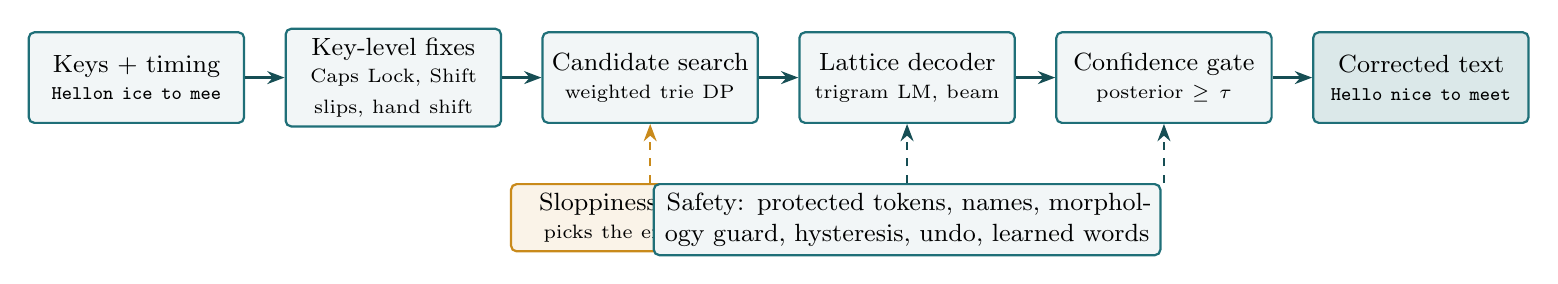
\begin{tikzpicture}[
  box/.style={draw=qkteal,rounded corners=2pt,thick,fill=qkteal!6,align=center,font=\small,minimum height=1.15cm,text width=2.5cm},
  arr/.style={-{Stealth[length=2.2mm]},thick,qkteal!70!black},
  node distance=0.5cm]
\node[box] (in) {Keys + timing\\[-1pt]\scriptsize\ttw{Hellon ice to mee}};
\node[box,right=of in] (pre) {Key-level fixes\\[-1pt]\scriptsize Caps Lock, Shift slips, hand shift};
\node[box,right=of pre] (cand) {Candidate search\\[-1pt]\scriptsize weighted trie DP};
\node[box,right=of cand] (lat) {Lattice decoder\\[-1pt]\scriptsize trigram LM, beam};
\node[box,right=of lat] (gate) {Confidence gate\\[-1pt]\scriptsize posterior $\geq\tau$};
\node[box,right=of gate,fill=qkteal!16] (out) {Corrected text\\[-1pt]\scriptsize\ttw{Hello nice to meet}};
\node[box,below=0.75cm of cand,text width=3.3cm,minimum height=0.85cm,fill=qkamber!10,draw=qkamber] (slop) {Sloppiness estimate\\[-1pt]\scriptsize picks the error model};
\node[box,below=0.75cm of lat,text width=6.2cm,minimum height=0.85cm] (safe) {Safety: protected tokens, names, morphology guard, hysteresis, undo, learned words};
\draw[arr] (in) -- (pre); \draw[arr] (pre) -- (cand); \draw[arr] (cand) -- (lat); \draw[arr] (lat) -- (gate); \draw[arr] (gate) -- (out);
\draw[arr,dashed,qkamber] (slop) -- (cand);
\draw[arr,dashed] (safe.north -| lat) -- (lat.south);
\draw[arr,dashed] (safe.north -| gate) -- (gate.south);
\end{tikzpicture}}
\caption{The \qk{} pipeline. Each chunk (the text between spaces) is decided when its space is pressed, so corrections are immediate. The last four chunks are then re-decoded jointly, so later words can fix earlier ones.}
\label{fig:pipeline}
\end{figure}

\subsection{Formulation}
For a typed chunk $t$ with key times $\mathbf{k}$ and context $c$, the decoder seeks
\begin{equation}
\hat{w} = \arg\max_{w \in \mathcal{H}(t)} \; P(t,\mathbf{k}\mid w)\; P(w \mid c).
\end{equation}
The hypothesis set $\mathcal{H}(t)$ contains:
\begin{itemize}
\item dictionary candidates;
\item run-together segmentations (\ttw{thecat} $\to$ \emph{the cat});
\item session-learned words;
\item a \emph{keep} hypothesis: the typed string is exactly what was meant.
\end{itemize}
Scores are costs in nats ($-\ln p$). For an unknown string, the keep cost is $\kappa_0 + \kappa_1\min(|t|,10)$. It makes long random strings unlikely as intentional words, while not penalising long genuine technical terms.

\subsection{Error model and candidate search}
Figure~\ref{fig:keyboard} illustrates the error model. A substitution costs more the farther apart the two keys are on a row-staggered QWERTY layout. An extra key is cheap when it repeats or neighbours an adjacent typed key. Dropping a doubled letter or an apostrophe is cheap. A transposition can be made cheaper when the two keys came within 45~ms (roll-over). Table~\ref{tab:channel} lists the costs.

Candidates come from running this weighted Damerau--Levenshtein recurrence directly over a trie of about 86,000 words, pruning any branch whose cheapest partial alignment exceeds a bound. The bound grows with word length, so long words can absorb more slips. A per-thread cache avoids repeating the search when a chunk is re-examined.

\begin{figure}[t]
\centering
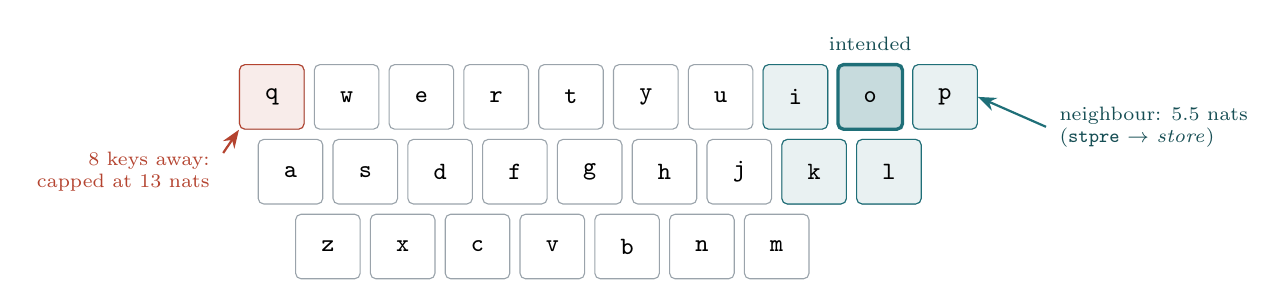
\begin{tikzpicture}[x=0.95cm,y=0.95cm]
\foreach \n/\x/\y in {q/0/0,w/1/0,e/2/0,r/3/0,t/4/0,y/5/0,u/6/0,i/7/0,o/8/0,p/9/0,a/0.25/-1,s/1.25/-1,d/2.25/-1,f/3.25/-1,g/4.25/-1,h/5.25/-1,j/6.25/-1,k/7.25/-1,l/8.25/-1,z/0.75/-2,x/1.75/-2,c/2.75/-2,v/3.75/-2,b/4.75/-2,n/5.75/-2,m/6.75/-2} {\node[draw=qkgrey,rounded corners=2pt,minimum size=0.82cm,font=\ttfamily\small] (k\n) at (\x,\y) {\n};}
% intended key and its neighbours
\node[draw=qkteal,very thick,fill=qkteal!25,rounded corners=2pt,minimum size=0.82cm,font=\ttfamily\small\bfseries] at (ko) {o};
\foreach \n in {i,p,k,l} {\node[draw=qkteal,fill=qkteal!10,rounded corners=2pt,minimum size=0.82cm,font=\ttfamily\small] at (k\n) {\n};}
\node[draw=qkred,fill=qkred!10,rounded corners=2pt,minimum size=0.82cm,font=\ttfamily\small] at (kq) {q};
\node[font=\scriptsize,qkteal!70!black,above=0.05cm of ko] {intended};
\node[font=\scriptsize,qkteal!70!black,align=left,anchor=west] at (10.4,-0.4) {neighbour: 5.5 nats\\(\ttw{stpre} $\to$ \emph{store})};
\node[font=\scriptsize,qkred,align=right,anchor=east] at (-0.7,-1.0) {8 keys away:\\capped at 13 nats};
\draw[-{Stealth},qkteal,thick] (10.35,-0.4) -- (kp.east);
\draw[-{Stealth},qkred,thick] (-0.65,-0.75) -- (kq.south west);
\end{tikzpicture}
\caption{The error model on a row-staggered QWERTY layout. Hitting a neighbour of the intended key (teal) is a common slip; a far key (red) is very unlikely. Costs are $-\ln p$: every 2.3 nats is a factor of 10.}
\label{fig:keyboard}
\end{figure}

\begin{table}[t]
\centering\small
\caption{Error-model costs in nats: default, and the profile fitted to the study participant (\S\ref{sec:real}).}
\label{tab:channel}
\begin{tabular}{lcc}
\toprule
Operation & Default & Fitted \\
\midrule
Substitution, adjacent key & 5.5 & 5.5 \\
\quad per extra key of distance & +3.0 & +2.0 \\
Extra key: repeat / adjacent / other & 5.5 / 6.0 / 11.0 & 5.5 / 6.0 / 7.0 \\
Missing letter: doubled / other & 4.0 / 6.5 & 4.0 / 4.5 \\
Transposition (fast / normal / slow) & 3.0 / 5.0 / 6.5 & 4.5 (no timing) \\
\bottomrule
\end{tabular}
\end{table}

\subsection{Language model}
Unigram frequencies combine Google Books counts via SymSpell~\citep{garbe2012symspell,michel2011} with \ttw{wordfreq}~\citep{speer2018wordfreq}, filtered for web misspellings (\S\ref{sec:lessons}). Bigram and trigram counts come from all 1.4~billion words of English Wiki-40B~\citep{guo2020wiki40b}, plus conversational text weighted up. The store holds 11.5M word pairs and 13M triples (62~MB). The context cost is
\begin{equation}
P(w\mid u,v) = \lambda_3\,\frac{c(u,v,w)}{c(u,v)} + (1-\lambda_3)\big[\lambda P_2(w\mid v) + (1-\lambda) P_1(w)\big],
\end{equation}
where $\lambda_3 = 0.7\,c(u,v)/(c(u,v)+5)$ and $\lambda=0.6$. Here $P_2$ takes the larger of the Google Books and corpus estimates, since each list misses pairs the other has.

\subsection{Sliding-window lattice decoder}
Deciding each word alone throws away information. \qk{} re-decodes the last four chunks as a lattice (Figure~\ref{fig:lattice}):
\begin{itemize}
\item \textbf{Single readings} for each chunk: keep, the top spelling candidates, splits, and learned words.
\item \textbf{Boundary readings} for each adjacent pair: a merge (\ttw{meetin g}), and the space moved one letter either way (\ttw{hellon ice}).
\end{itemize}
A beam search over states of the last two words~\citep{rabiner1989} finds the best path under the trigram model.

\begin{figure}[t]
\centering
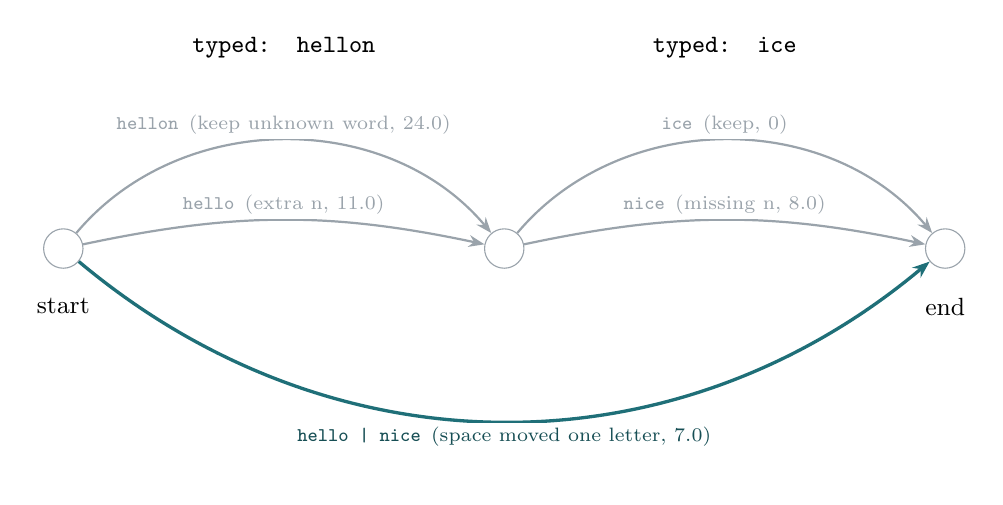
\begin{tikzpicture}[
  st/.style={circle,draw=qkgrey,fill=white,minimum size=5mm,inner sep=0},
  rd/.style={font=\scriptsize\ttfamily,fill=white,inner sep=1.5pt},
  edge/.style={-{Stealth[length=2mm]},qkgrey,thick},
  best/.style={-{Stealth[length=2.2mm]},qkteal,very thick}]
\node[st] (s0) at (0,0) {};
\node[st] (s1) at (5.6,0) {};
\node[st] (s2) at (11.2,0) {};
\node[font=\small,below=0.25cm of s0] {start};
\node[font=\small,below=0.25cm of s2] {end};
\node[font=\small\ttfamily,above=2.3cm of $(s0)!0.5!(s1)$] {typed: hellon};
\node[font=\small\ttfamily,above=2.3cm of $(s1)!0.5!(s2)$] {typed: ice};
% single readings chunk 1
\draw[edge] (s0) to[bend left=50] node[rd,above] {hellon \textrm{(keep unknown word, 24.0)}} (s1);
\draw[edge] (s0) to[bend left=12] node[rd,above] {hello \textrm{(extra n, 11.0)}} (s1);
% single readings chunk 2
\draw[edge] (s1) to[bend left=50] node[rd,above] {ice \textrm{(keep, 0)}} (s2);
\draw[edge] (s1) to[bend left=12] node[rd,above] {nice \textrm{(missing n, 8.0)}} (s2);
% pair reading
\draw[best] (s0) to[bend right=40] node[rd,below,text=qkteal!70!black] {hello | nice \textrm{(space moved one letter, 7.0)}} (s2);
\end{tikzpicture}
\caption{A lattice over two typed chunks. Grey arcs are single-chunk readings, and the teal arc is a boundary reading that moves the space. Each arc's error cost (nats) is shown; the language model adds a cost for every word along the path. Moving the space (7.0) explains the typing far more cheaply than two separate slips (11.0 + 8.0), and the single-chunk path through \emph{hello} and \emph{nice} produces the same text, adding to its probability.}
\label{fig:lattice}
\end{figure}

\paragraph{Path-summed confidence.} A change at chunk $k$ is applied only if its posterior clears a threshold:
\begin{equation}
P(\text{text}_k = y) = \frac{\sum_{\pi:\,\text{text}_k(\pi)=y} e^{-S(\pi)}}{\sum_{\pi} e^{-S(\pi)}} \;\geq\; \tau,
\end{equation}
computed with a beam-pruned forward pass. The thresholds are $\tau=0.9$ for non-words, and $0.98$ (plus a 1.5-nat cost) for changing a real word. Summing over paths matters. An earlier version compared the best path against the best competing path, and refused \ttw{th efriend}~$\to$~\emph{the friend}, because two different paths produce that text (move the space, or drop the stray \ttw{e}) and each made the other look like a rival (Figure~\ref{fig:pathsum}).

\begin{figure}[t]
\centering
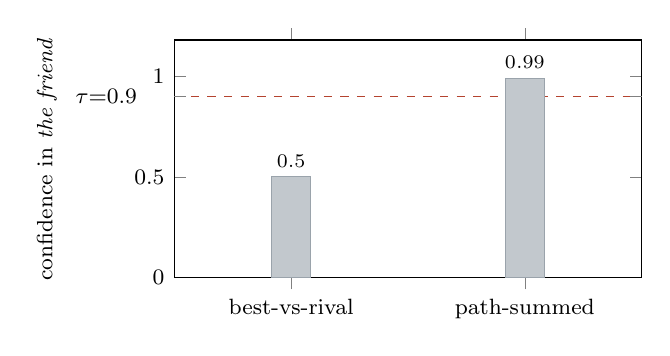
\begin{tikzpicture}
\begin{axis}[ybar,bar width=14pt,width=0.62\linewidth,height=4.6cm,ymin=0,ymax=1.18,ytick={0,0.5,1},
  symbolic x coords={best-vs-rival,path-summed},xtick=data,ylabel={confidence in \emph{the friend}},
  nodes near coords,nodes near coords style={font=\scriptsize},every node near coord/.append style={/pgf/number format/fixed,/pgf/number format/precision=2},
  tick label style={font=\footnotesize},label style={font=\footnotesize},enlarge x limits=0.5,
  extra y ticks={0.9},extra y tick style={grid=major,grid style={qkred,dashed},tick label style={xshift=-0.35cm}},extra y tick labels={$\tau{=}0.9$}]
\addplot[fill=qkgrey!60,draw=qkgrey] coordinates {(best-vs-rival,0.50) (path-summed,0.99)};
\end{axis}
\end{tikzpicture}
\caption{Why confidence must sum over paths, for \ttw{th efriend}. Two paths produce \emph{the friend}. Comparing the best path with its best rival splits the evidence about 50/50, below the threshold $\tau$; summing paths by output text gives about 0.99. Values are illustrative of the measured behaviour.}
\label{fig:pathsum}
\end{figure}

\subsection{Safety mechanisms}
\label{sec:safety}
\begin{itemize}
\item \textbf{Protected tokens} are never touched: digits, \ttw{snake\_case}, \ttw{camelCase}, paths, URLs, e-mail addresses, flags (\ttw{--force}), ALL-CAPS acronyms, dialect elisions (\ttw{countin'}) and abbreviations (\ttw{Mr.}).
\item \textbf{Names.} An unknown capitalised word mid-sentence needs 99.9\% confidence. It may be fixed toward a known proper noun only if the slip is a single clean keyboard slip, not in the first letter. This separates \ttw{Calicornia}~$\to$~\emph{California} from \ttw{Colman}~$\to$~\emph{Coleman}: names differ by spelling-variant patterns, typos by keyboard patterns. Words normally capitalised, learned from Wikipedia casing, are restored (\ttw{london}~$\to$~\emph{London}).
\item \textbf{Morphology guard.} A known stem plus a regular affix (\ttw{freewheelers}) is treated as a real word.
\item \textbf{Hysteresis.} A word changes at most once. The only exception is a boundary repair, which may override an earlier spelling fix.
\item \textbf{Undo and learning.} Undoing a correction protects the word and learns it. So does typing a word identically twice. Later typos of learned words are fixed toward them (\ttw{kubetcl}~$\to$~\emph{kubectl}).
\item \textbf{English variety.} When a typo is corrected and both UK and US forms exist (1,115 pairs), the preferred variety (UK by default) wins. Correctly typed words are never changed.
\end{itemize}

\subsection{Errors beyond letters}
\label{sec:special}
\begin{itemize}
\item \textbf{Spacing.} Missing spaces are handled by segmentation, with exact pieces or one fuzzy piece. Premature and shifted spaces are handled by boundary readings. Merging two real words requires 6 extra nats of evidence, because merges are how compounds get mangled (\ttw{soy beans}).
\item \textbf{Hand shift.} A word typed one key over (\ttw{jr;;p}~$\to$~\emph{hello}) is detected by remapping it.
\item \textbf{Shift slips.} Patterns such as \ttw{THe}, \ttw{hTe} and \ttw{uSre}~$\to$~\emph{Sure} are recognised: a capital in second position means the first two keys rolled over.
\item \textbf{Accidental Caps Lock.} Three inverted-case words in a row (\ttw{w NEED TO}) switch on case flipping, including mistimed Shift under Caps Lock (\ttw{thANSK}~$\to$~\emph{Thanks}). Real acronyms do not trigger it.
\end{itemize}

\subsection{Adapting to sloppiness}
Rough aim needs a different error model: adjacent slips cheap, distant keys steep. \qk{} estimates sloppiness online as the share of the last 50 words typed as non-words. It switches to the rough-aim model above 45\% and back below 35\% (Figure~\ref{fig:sloppy}).

\begin{figure}[t]
\centering
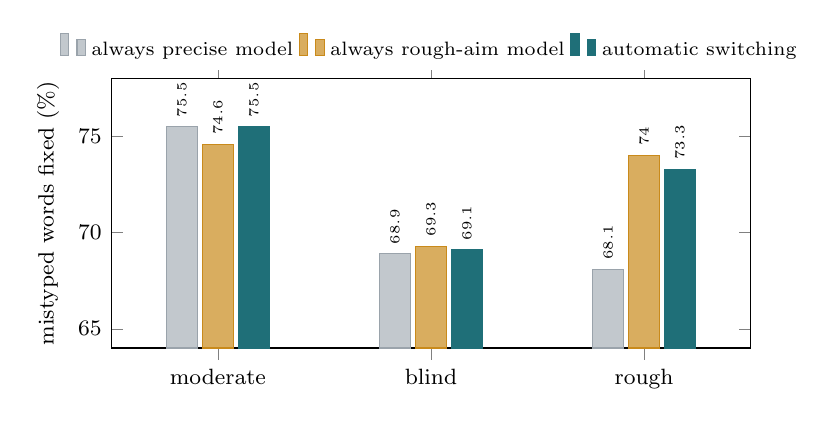
\begin{tikzpicture}
\begin{axis}[ybar,bar width=11pt,width=0.8\linewidth,height=5cm,ymin=64,ymax=78,
  symbolic x coords={moderate,blind,rough},xtick=data,ylabel={mistyped words fixed (\%)},
  legend style={font=\scriptsize,at={(0.5,1.03)},anchor=south,legend columns=3,draw=none},
  tick label style={font=\footnotesize},label style={font=\footnotesize},enlarge x limits=0.25,
  nodes near coords,nodes near coords style={font=\tiny,rotate=90,anchor=west},every node near coord/.append style={/pgf/number format/fixed,/pgf/number format/precision=1}]
\addplot[fill=qkgrey!60,draw=qkgrey] coordinates {(moderate,75.5) (blind,68.9) (rough,68.1)};
\addplot[fill=qkamber!70,draw=qkamber] coordinates {(moderate,74.6) (blind,69.3) (rough,74.0)};
\addplot[fill=qkteal,draw=qkteal] coordinates {(moderate,75.5) (blind,69.1) (rough,73.3)};
\legend{always precise model,always rough-aim model,automatic switching}
\end{axis}
\end{tikzpicture}
\caption{Switching error models by measured sloppiness (whole documents, development data). The switch keeps careful typing on the precise model and gives rough typing most of the rough-aim model's 5-point gain.}
\label{fig:sloppy}
\end{figure}

%=====================================================================
\section{Evaluation Methodology}
\label{sec:eval}

\paragraph{Text.} Clean sentences come from the Brown corpus~\citep{francis1979}, which is independent of all the engine's data sources. There are 1,500 development sentences for all tuning, 1,500 held-out test sentences for reporting, and 60 whole documents for document-level effects.

\paragraph{Simulated typist.} A simulated typist types the clean text. The discrete-slip model mixes:
\begin{itemize}
\item adjacent-key substitutions;
\item transpositions, with short inter-key intervals (which also occur on 6\% of correct pairs, so timing is a hint and not a give-away);
\item omissions, fat-finger presses and double taps;
\item missing, premature and shifted spaces, and whole-hand shifts.
\end{itemize}
The \emph{rough-aim} model lands every press at a Gaussian offset around the intended key ($\sigma=0.30$ key widths horizontally, 0.24 vertically), with roll-overs and drops on top. Table~\ref{tab:levels} lists the levels.

\begin{table}[t]
\centering\small
\caption{Simulated typing levels.}
\label{tab:levels}
\begin{tabular}{lccl}
\toprule
Level & Letters mistyped & Words mistyped & \\
\midrule
light & 1.5\% & 7\% & careful typist \\
moderate & 3\% & 14\% & \\
messy & 6\% & 26\% & \\
blind & 10\% & 38\% & not looking at the keys \\
rough & Gaussian aim & 49\% & the north star \\
\bottomrule
\end{tabular}
\end{table}

\paragraph{Metrics.} For mistyped words we report the share \emph{fixed}, changed to the \emph{wrong} word, or \emph{left} as typed. For correctly typed words we report the \emph{false-correction} rate, the number that decides whether people keep a corrector on. Word accuracy is the share of words output exactly right. Latency is per word on one CPU core.

\paragraph{Baseline.} \emph{plain} is a frequency-only spellchecker built from the same parts, without geometry, timing, context, splits or the lattice. We could not run operating-system autocorrect in our environment (\S\ref{sec:limits}).

%=====================================================================
\section{Results on Simulated Typing}

Figure~\ref{fig:simacc} and Table~\ref{tab:main} give the held-out results. \qk{} fixes 24--34 points more mistyped words than the baseline at every level, with false corrections of about one in 750 correctly typed words.

\begin{figure}[t]
\centering
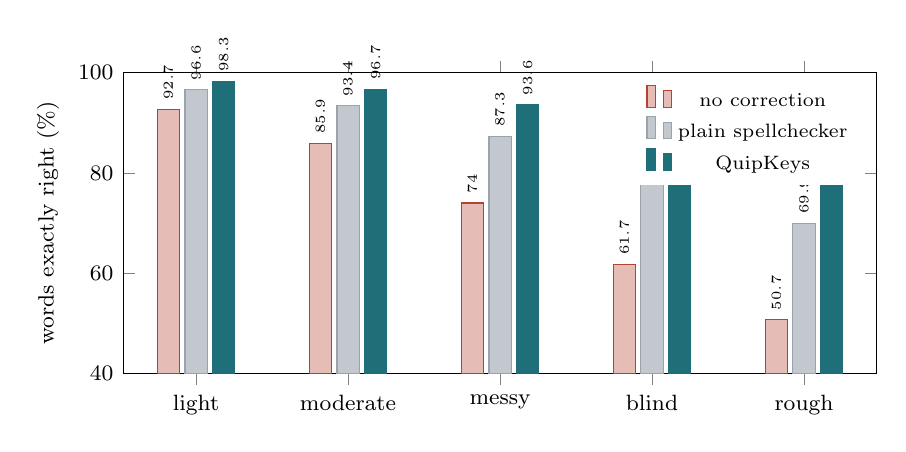
\begin{tikzpicture}
\begin{axis}[ybar,bar width=8pt,width=0.92\linewidth,height=5.4cm,ymin=40,ymax=100,
  symbolic x coords={light,moderate,messy,blind,rough},xtick=data,ylabel={words exactly right (\%)},
  legend style={font=\scriptsize,at={(0.98,0.98)},anchor=north east,draw=none},
  tick label style={font=\footnotesize},label style={font=\footnotesize},enlarge x limits=0.12,
  nodes near coords,nodes near coords style={font=\tiny,rotate=90,anchor=west},every node near coord/.append style={/pgf/number format/fixed,/pgf/number format/precision=1}]
\addplot[fill=qkred!35,draw=qkred] coordinates {(light,92.7) (moderate,85.9) (messy,74.0) (blind,61.7) (rough,50.7)};
\addplot[fill=qkgrey!60,draw=qkgrey] coordinates {(light,96.6) (moderate,93.4) (messy,87.3) (blind,79.7) (rough,69.9)};
\addplot[fill=qkteal,draw=qkteal] coordinates {(light,98.3) (moderate,96.7) (messy,93.6) (blind,89.0) (rough,86.6)};
\legend{no correction,plain spellchecker,\qk}
\end{axis}
\end{tikzpicture}
\caption{Word accuracy on held-out simulated typing. The sloppier the typing, the larger \qk{}'s margin over a spellchecker.}
\label{fig:simacc}
\end{figure}

\begin{table}[t]
\centering\small
\caption{Held-out simulated typing (1,500 Brown test sentences per level).}
\label{tab:main}
\begin{tabular}{llccccc}
\toprule
Level & System & Fixed & Wrong & False corr. & Word acc. & p50 / p99 (ms) \\
\midrule
light & no correction & -- & -- & -- & 92.72\% & -- \\
 & plain & 55.0\% & 2.5\% & 0.095\% & 96.64\% & 0.3 / 2.8 \\
 & \qk{} & 78.7\% & 2.0\% & 0.135\% & 98.33\% & 0.5 / 3.1 \\
\addlinespace
moderate & no correction & -- & -- & -- & 85.92\% & -- \\
 & plain & 53.5\% & 3.3\% & 0.078\% & 93.39\% & 0.4 / 3.1 \\
 & \qk{} & 77.3\% & 2.4\% & 0.132\% & 96.69\% & 0.6 / 4.0 \\
\addlinespace
messy & no correction & -- & -- & -- & 73.98\% & -- \\
 & plain & 51.3\% & 3.9\% & 0.080\% & 87.27\% & 0.6 / 3.8 \\
 & \qk{} & 75.5\% & 3.3\% & 0.109\% & 93.55\% & 0.8 / 5.3 \\
\addlinespace
blind & no correction & -- & -- & -- & 61.74\% & -- \\
 & plain & 46.9\% & 4.8\% & 0.076\% & 79.65\% & 0.8 / 4.3 \\
 & \qk{} & 71.5\% & 4.1\% & 0.125\% & 89.03\% & 1.0 / 8.3 \\
\addlinespace
rough & no correction & -- & -- & -- & 50.71\% & -- \\
 & plain & 39.1\% & 5.6\% & 0.076\% & 69.92\% & 0.9 / 4.7 \\
 & \qk{} & 72.9\% & 4.1\% & 0.135\% & 86.55\% & 1.2 / 9.9 \\
\bottomrule
\end{tabular}

\end{table}

\paragraph{Ablations.} Table~\ref{tab:ablate} switches components off one at a time.
\begin{itemize}
\item \textbf{Keyboard geometry} is the most valuable single component: 5--6 points, and 17 under rough aim.
\item \textbf{Trigram context} and \textbf{boundary repair} each add about 3 points.
\item \textbf{The lattice decoder} adds 0.2--2 points.
\item \textbf{The rough-aim error model} adds 3.5 points on rough typing.
\end{itemize}

\begin{table}[t]
\centering\small
\caption{Ablations: share of mistyped words fixed (held-out simulated typing).}
\label{tab:ablate}
\begin{tabular}{lcccc}
\toprule
Configuration & moderate & messy & blind & rough \\
\midrule
\qk{} (full) & 77.3\% & 75.5\% & 71.5\% & 72.9\% \\\midrule
word-by-word instead of lattice & 77.1\% & 74.5\% & 70.2\% & 70.7\% \\
no keyboard geometry & 72.3\% & 70.5\% & 65.2\% & 56.0\% \\
pairs only (no trigrams) & 74.0\% & 72.8\% & 68.7\% & 69.9\% \\
no boundary repair & 74.4\% & 72.2\% & 68.6\% & 70.5\% \\
never switch to rough-aim model & 77.3\% & 75.5\% & 71.1\% & 69.4\% \\
plain (frequency-only) & 53.5\% & 51.3\% & 46.9\% & 39.1\% \\
\bottomrule
\end{tabular}

\end{table}

%=====================================================================
\section{Real Typing}
\label{sec:real}

\paragraph{Protocol.} One participant, the author, typed 33 thirty-word passages of everyday sentences in a browser-based Typing Lab, which logged every keystroke with millisecond timing and applied no correction. All runs used the north-star condition: as fast as possible, not looking, backspace disabled. Most hid the typed text, because seeing it prompted the participant to go back and fix. Five early runs were typed with Caps Lock on by accident. Logs were replayed through the engine and scored on words, ignoring case and punctuation, since the participant mostly omitted punctuation.

\paragraph{Accuracy.} Words typed exactly right rose from 75.4\% to 91.5\% (Figure~\ref{fig:real}). Every run improved, and three reached 96--100\%. At the median raw speed of 85~WPM, that is roughly 64 correct words per minute uncorrected versus 78 with \qk. On the 21 runs typed after the personal error model was fitted, the engine scored 92.4\%, or 93.0\% with the fitted model.

\begin{figure}[t]
\centering
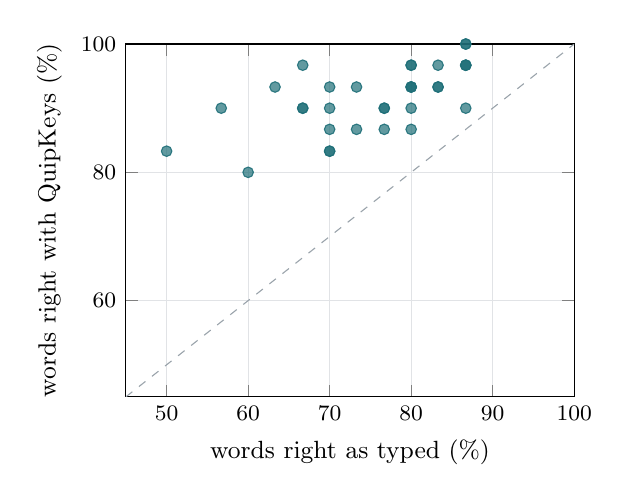
\begin{tikzpicture}
\begin{axis}[width=0.6\linewidth,height=0.5\linewidth,
  xlabel={words right as typed (\%)},ylabel={words right with \qk{} (\%)},
  xmin=45,xmax=100,ymin=45,ymax=100,grid=major,grid style={qkgrey!30},
  tick label style={font=\footnotesize},label style={font=\small}]
\addplot[qkgrey,dashed,domain=45:100] {x};
\addplot[only marks,mark=*,mark size=1.9pt,qkteal,fill opacity=0.7,draw opacity=0.9] coordinates {
(80.0,96.7) (80.0,93.3) (66.7,90.0) (83.3,93.3) (70.0,86.7) (80.0,93.3) (80.0,90.0) (76.7,90.0) (80.0,93.3) (50.0,83.3) (80.0,86.7) (70.0,83.3) (70.0,83.3) (76.7,86.7) (56.7,90.0) (86.7,100.0) (73.3,93.3) (86.7,96.7) (63.3,93.3) (80.0,96.7) (83.3,93.3) (70.0,93.3) (76.7,90.0) (73.3,86.7) (66.7,90.0) (86.7,96.7) (86.7,100.0) (86.7,90.0) (70.0,90.0) (83.3,96.7) (86.7,96.7) (60.0,80.0) (66.7,96.7)};
\end{axis}
\end{tikzpicture}
\caption{Real typing, one point per 30-word run (33 runs, 75--96~WPM, not looking, no backspace). Every run lies above the diagonal.}
\label{fig:real}
\end{figure}

\paragraph{The real error profile.} Figure~\ref{fig:profile} compares the participant's 346 slips with the simulator's assumptions. Two assumptions were wrong:
\begin{enumerate}
\item Most extra letters are \emph{not} neighbours of the keys around them (66 of 100).
\item Swapped pairs happen at normal pace (about 100--150~ms between keys), not as sub-45~ms roll-overs.
\end{enumerate}

\begin{figure}[t]
\centering
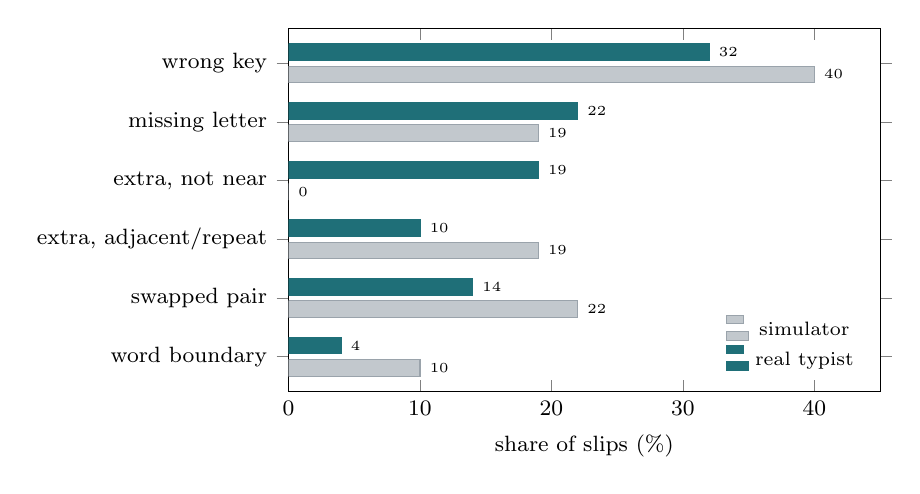
\begin{tikzpicture}
\begin{axis}[xbar,bar width=6pt,width=0.75\linewidth,height=6.2cm,xmin=0,xmax=45,
  symbolic y coords={word boundary,swapped pair,{extra, adjacent/repeat},{extra, not near},missing letter,wrong key},ytick=data,
  xlabel={share of slips (\%)},legend style={font=\scriptsize,at={(0.98,0.03)},anchor=south east,draw=none},
  tick label style={font=\footnotesize},label style={font=\footnotesize},enlarge y limits=0.12,
  nodes near coords,nodes near coords style={font=\tiny},every node near coord/.append style={/pgf/number format/fixed,/pgf/number format/precision=0}]
\addplot[fill=qkgrey!60,draw=qkgrey] coordinates {(10,word boundary) (22,swapped pair) (19,{extra, adjacent/repeat}) (0,{extra, not near}) (19,missing letter) (40,wrong key)};
\addplot[fill=qkteal,draw=qkteal] coordinates {(4,word boundary) (14,swapped pair) (10,{extra, adjacent/repeat}) (19,{extra, not near}) (22,missing letter) (32,wrong key)};
\legend{simulator,real typist}
\end{axis}
\end{tikzpicture}
\caption{Where the slips came from: real typist (33 runs, 3,944 letters, 8.8\% mistyped) versus the discrete-slip simulator. The simulator had no extra letters away from neighbouring keys, the real typist's most distinctive slip.}
\label{fig:profile}
\end{figure}

\paragraph{Ablations on real typing.} Figure~\ref{fig:ablreal} shows the decisive difference between simulated and real typing. Keyboard geometry, the most valuable component in simulation, contributed nothing on real typing. Context and boundary repair carried the gains, and a frequency-only spellchecker reached 84.7\%.

\begin{figure}[t]
\centering
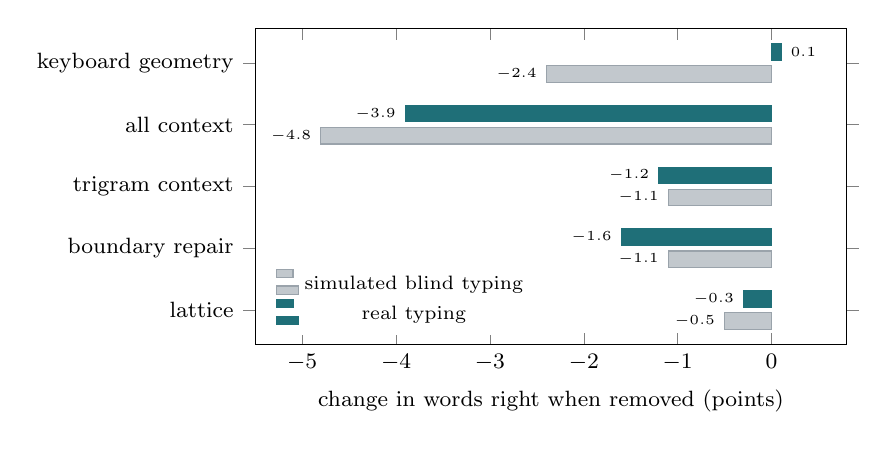
\begin{tikzpicture}
\begin{axis}[xbar,bar width=6pt,width=0.75\linewidth,height=5.6cm,xmin=-5.5,xmax=0.8,
  symbolic y coords={lattice,boundary repair,trigram context,all context,keyboard geometry},ytick=data,
  xlabel={change in words right when removed (points)},legend style={font=\scriptsize,at={(0.02,0.03)},anchor=south west,draw=none},
  tick label style={font=\footnotesize},label style={font=\footnotesize},enlarge y limits=0.14,
  nodes near coords,nodes near coords style={font=\tiny},every node near coord/.append style={/pgf/number format/fixed,/pgf/number format/precision=1}]
\addplot[fill=qkgrey!60,draw=qkgrey] coordinates {(-0.5,lattice) (-1.1,boundary repair) (-1.1,trigram context) (-4.8,all context) (-2.4,keyboard geometry)};
\addplot[fill=qkteal,draw=qkteal] coordinates {(-0.3,lattice) (-1.6,boundary repair) (-1.2,trigram context) (-3.9,all context) (0.1,keyboard geometry)};
\legend{simulated blind typing,real typing}
\end{axis}
\end{tikzpicture}
\caption{Removing each component, simulated blind typing versus real typing (word accuracy). On real typing, removing geometry changes nothing; context matters most.}
\label{fig:ablreal}
\end{figure}

\paragraph{Fitted error model.} Re-estimating the error costs from the real profile (Table~\ref{tab:channel}) gained 1.7 points on the 12 runs it was fitted to, and 0.6 points on the 21 runs typed afterwards. The gain is small but it generalises. It is opt-in for now, because cheaper extra and missing letters widen the search and slow the worst case.

%=====================================================================
\section{A Neural Language Model}
\label{sec:nn}

Half of the words still wrong on real typing are \emph{real-word} slips: \ttw{ship} for \emph{shop}, \ttw{our}/\ttw{out}, \ttw{nice} for \emph{nine}, \ttw{quite}/\ttw{quiet}, \ttw{fat}/\ttw{far}. Trigram context cannot overrule these safely, so we trained a neural language model.

\paragraph{Model and training.} The model is a 6-layer, 6-head decoder-only transformer with 384 dimensions and 23.3M parameters. Its word-level vocabulary is the engine's 32,768 most frequent words plus unknown-word and boundary tokens, with 64-word context and tied input/output embeddings. Training text was 32 Wiki-40B files plus conversational text weighted up: 398.9M tokens, tokenised with the engine's own tokeniser. Training ran for 110,000 steps (batch 64), about 3 hours on an RTX~2060 at about 55k tokens/s, reaching validation perplexity 59. A CPU proof of concept (4.6M parameters, 1 hour) had reached about 200. The exported weights are int8 with per-row scales, and inference is pure Rust with an incremental key-value cache.

\paragraph{Two ways to use it.}
\begin{enumerate}
\item As a \emph{left-context re-ranker}: each chunk's readings get $\alpha(\mathrm{lse}-\mathrm{logit})$ added, using the model's next-word logits given everything before the chunk.
\item As a \emph{look-ahead} for real words: two words after a real word is typed, each one-slip real-word alternative is tried in place, and the model scores the alternative plus the following words with a full softmax.
\end{enumerate}

\paragraph{Results.} Figure~\ref{fig:nn} shows the outcome. On real typing it gave at most +0.3 points. The look-ahead changed no outputs at all. On simulated typing the re-ranker doubled real-word fixes (8\% to 17\%), but cost about a point overall, raised false corrections, and was 50$\times$ slower (18~ms median per word, unoptimised).

\begin{figure}[t]
\centering
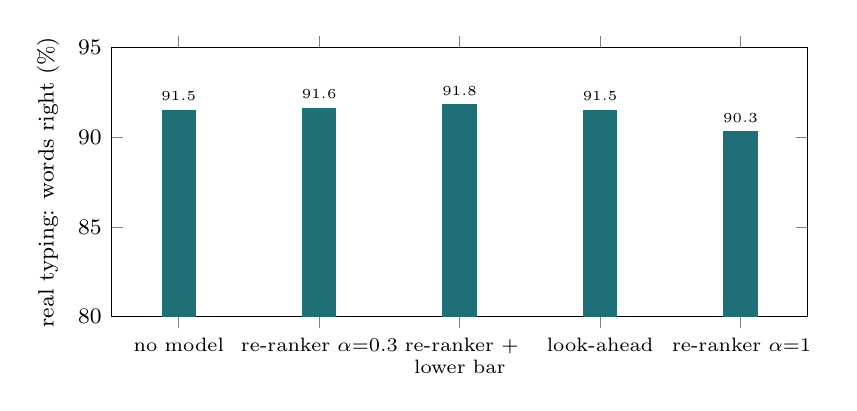
\begin{tikzpicture}
\begin{axis}[ybar,bar width=12pt,width=0.86\linewidth,height=5cm,ymin=80,ymax=95,
  symbolic x coords={no model,re-ranker $\alpha{=}0.3$,re-ranker + lower bar,look-ahead,re-ranker $\alpha{=}1$},xtick=data,
  ylabel={real typing: words right (\%)},x tick label style={font=\scriptsize,align=center,text width=2cm},
  tick label style={font=\footnotesize},label style={font=\footnotesize},enlarge x limits=0.12,
  nodes near coords,nodes near coords style={font=\tiny},every node near coord/.append style={/pgf/number format/fixed,/pgf/number format/precision=1}]
\addplot[fill=qkteal,draw=qkteal] coordinates {(no model,91.5) (re-ranker $\alpha{=}0.3$,91.6) (re-ranker + lower bar,91.8) (look-ahead,91.5) (re-ranker $\alpha{=}1$,90.3)};
\end{axis}
\end{tikzpicture}
\caption{The 23M-parameter neural language model on real typing (33 runs). At best it adds 0.3 points; at full weight it hurts.}
\label{fig:nn}
\end{figure}

\paragraph{Why it did not help.} We scored each candidate together with the words after it. The model's preferences were usually right, but the evidence was weak or too far away (Table~\ref{tab:nnpairs}):
\begin{itemize}
\item \emph{our}~$\to$~\emph{out} gets 13.6 nats, and is fixed.
\item \emph{fat}~$\to$~\emph{far} gets 3.6 nats, and \emph{quite}~$\to$~\emph{quiet} 2.1. That is not enough to overcome the roughly 7-nat prior against a one-slip real-word error (a neighbouring-key slip that lands on another valid word).
\item For \emph{ship}~$\to$~\emph{shop} the model has no preference: the disambiguating word (\emph{closes}) is three words away.
\end{itemize}
In the participant's real typing, the words after a real-word slip are often misspelled themselves, which weakens the evidence further. Lowering the prior to let 2--4 nats through would also flip correct words, the failure the system exists to avoid.

\begin{table}[t]
\centering\small
\caption{Neural evidence for real-word alternatives: log-probability of (candidate + following words) given the preceding words, as the advantage in nats of the intended word over the typed one.}
\label{tab:nnpairs}
\begin{tabular}{llcl}
\toprule
Context & Typed $\to$ intended & Evidence & Outcome \\
\midrule
\emph{thanks for helping \_ with the} & our $\to$ out & +13.6 & fixed \\
\emph{ate \_ too much popcorn} & fat $\to$ far & +3.6 & below the bar \\
\emph{it was nice and \_ in the} & quite $\to$ quiet & +2.1 & below the bar \\
\emph{go to the \_ before it closes} & ship $\to$ shop & +0.0 & no preference \\
\bottomrule
\end{tabular}
\end{table}

\paragraph{Interpretation.} The remaining errors are short of \emph{information}, not intelligence. A bigger model would sharpen preferences such as \emph{far}/\emph{fat}, but cannot invent evidence that the keystrokes and nearby words do not contain (\S\ref{sec:future}).

%=====================================================================
\section{What Remains, and Lessons}
\label{sec:lessons}

\begin{figure}[t]
\centering
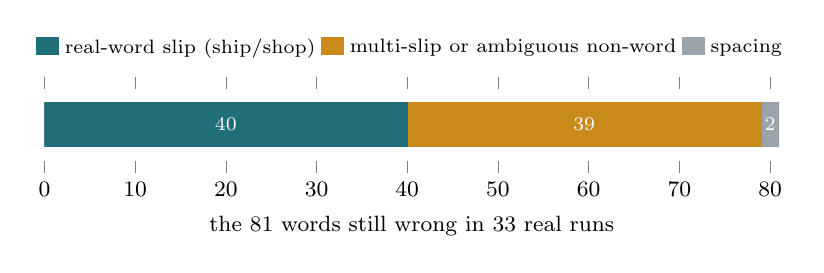
\begin{tikzpicture}
\begin{axis}[xbar stacked,bar width=16pt,width=0.9\linewidth,height=2.8cm,xmin=0,xmax=81,
  ytick=\empty,xlabel={the 81 words still wrong in 33 real runs},axis line style={draw=none},
  tick label style={font=\footnotesize},label style={font=\footnotesize},
  legend style={font=\scriptsize,at={(0.5,1.08)},anchor=south,legend columns=3,draw=none},
  nodes near coords,nodes near coords style={font=\scriptsize,color=white}]
\addplot[fill=qkteal,draw=qkteal] coordinates {(40,0)};
\addplot[fill=qkamber,draw=qkamber] coordinates {(39,0)};
\addplot[fill=qkgrey,draw=qkgrey] coordinates {(2,0)};
\legend{real-word slip (ship/shop),multi-slip or ambiguous non-word,spacing}
\end{axis}
\end{tikzpicture}
\caption{What is left. Half the remaining errors are real-word slips, which need evidence the context rarely provides; half are badly garbled or genuinely ambiguous.}
\label{fig:remaining}
\end{figure}

Of the 81 words still wrong across the 33 real runs (Figure~\ref{fig:remaining}):
\begin{itemize}
\item 49\% are real-word slips (\S\ref{sec:nn});
\item 48\% are non-words with two or more slips, or genuinely ambiguous readings (\ttw{asn}: \emph{and} or \emph{an}? \ttw{thei}: \emph{this}, \emph{their} or \emph{the}?);
\item 2\% are spacing errors.
\end{itemize}

\paragraph{Negative results.}
\begin{itemize}
\item \textbf{4-grams.} 6.6M 4-grams from the same 1.4B words gave no gain and more false corrections.
\item \textbf{A learned decision gate.} A logistic model over 18 decision features improved its training objective, but raised false corrections on the benchmark. It was not adopted.
\item \textbf{A document word cache} reinforced uncorrected slips. It was replaced by learning only words typed identically twice, which adds 0.1--0.3 points on documents.
\end{itemize}

\paragraph{Dictionary hygiene.} A rule admitting UK/US variant pairs (\ttw{enrolment}/\ttw{enrollment}) also admitted 364 web misspellings (\ttw{actualy}, \ttw{realy}, \ttw{allready}) as words. Real variants are within about 10$\times$ of each other in frequency; misspellings are 300--3000$\times$ rarer than their word. A frequency-ratio filter separates them. The participant's own typing (\ttw{actyaly}) exposed the bug; the simulator never could.

%=====================================================================
\section{Limitations}
\label{sec:limits}
\begin{itemize}
\item \textbf{One participant}, who is also the author. The held-out split guards against fitting to particular runs, not to a particular person.
\item \textbf{No comparison with operating-system autocorrect.} The baseline is our own frequency-only spellchecker.
\item \textbf{The key behavioural question is unmeasured:} does fast, sloppy typing with \qk{} beat careful typing with backspace? The participant's careful baseline was not recorded.
\item \textbf{The simulator is partly wrong} for this typist (Figure~\ref{fig:profile}), so simulated results should be read with that in mind.
\item \textbf{The evaluation text} is 1960s American prose, while the engine prefers UK spellings.
\item \textbf{No operating-system integration yet.}
\end{itemize}

%=====================================================================
\section{Future Work: More Information, Not More Intelligence}
\label{sec:future}
The analysis in \S\ref{sec:nn} points to supplying new evidence rather than larger models:
\begin{itemize}
\item \textbf{Key-up timing.} Physical keyboards report key-up as well as key-down. Extra letters are this typist's most distinctive slip, and accidental brushes may show unusually short hold times or overlap with neighbouring presses. That signal is free, and invisible in text.
\item \textbf{Personal text.} A language model adapted to the user's own writing (their phrases, names and topics) gives exactly the context that general text lacks.
\item \textbf{Interaction instead of guessing.} For an uncertain real word, underline it and let the user accept a suggestion with one key. A one-key fix still beats retyping, and nothing is silently changed.
\item \textbf{Online personal error models,} learned from accepted and undone corrections.
\item \textbf{A proper study:} careful typing, sloppy typing with \qk{}, and sloppy typing with built-in autocorrect, with more participants, including typists with motor impairments, for whom imprecision is not a choice.
\end{itemize}

\section{Conclusion}
Phone-style decoding transfers to physical keyboards. On real blind typing at 85~WPM, \qk{} raised exact-word accuracy from 75\% to over 91\% while rarely touching correct text. Real data was decisive throughout. It corrected the simulator, found a dictionary bug, and showed that context, not geometry, carries the gains for this typist. A neural language model trained for the remaining real-word slips confirmed that those errors are limited by missing information. The next gains will come from new signals (timing, personal text) and from interaction design, not from more model capacity.

\paragraph{Acknowledgements.} The engine, benchmark, data-collection tools and this report were developed with the help of Claude, an AI assistant by Anthropic.

\bibliographystyle{plainnat}
\bibliography{refs}
\end{document}
